\documentclass[preprint,12pt,authoryear]{elsarticle}
\usepackage{amsmath,amssymb,booktabs,array,graphicx,float,placeins,setspace,tabularx}
\usepackage[T1]{fontenc}
\usepackage[utf8]{inputenc}
\usepackage{lmodern,microtype}
\usepackage{xurl}
\usepackage[colorlinks=true,citecolor=blue,linkcolor=blue,urlcolor=black]{hyperref}
\journal{Journal of Forecasting}
\setlength{\emergencystretch}{2em}
\setlength{\textfloatsep}{10pt plus 2pt minus 2pt}
\setlength{\floatsep}{9pt plus 2pt minus 2pt}
\setlength{\intextsep}{9pt plus 2pt minus 2pt}
\setlength{\abovecaptionskip}{6pt}
\setlength{\belowcaptionskip}{2pt}
\graphicspath{{figures/}}

\begin{document}
\begin{frontmatter}

\title{Forecast Evaluation with Constructed High-Frequency Targets:
Information-Set Leakage and an African Gross Domestic Product Application}
\author[caperc]{Emmanuel Akande\corref{cor1}\fnref{orcid1}}
\ead{eakande@capeeconomicconsult.com}
\author[caperc]{Shakir Tewogbade}
\author[cbn]{Temitope J. Laniran}
\author[cbn]{Elijah Akanni}
\author[caperc]{Oyedamola Funmibi Taiwo}
\author[ui]{Honey Adenike Adeleke}
\author[ui]{Kafayat Ajoke Alobaloke}

\cortext[cor1]{Corresponding author: Emmanuel Akande, CAPE Economic Research and Consulting, 11120 Godwit Ln, Charlotte, NC 28278, USA.}
\fntext[orcid1]{ORCID: \url{https://orcid.org/0000-0002-8201-4072}.}
\address[caperc]{CAPE Economic Research and Consulting, 11120 Godwit Ln, Charlotte, NC 28278, USA}
\address[cbn]{Central Bank of Nigeria, Plot 33, Abubakar Tafawa Balewa Way, Central Business District, Abuja, Federal Capital Territory, Nigeria}
\address[ui]{University of Ibadan, Ibadan, Oyo State, Nigeria}


\begin{abstract}
Forecast studies sometimes evaluate monthly or quarterly predictions against targets reconstructed from annual data. A problem arises when the same final-vintage reconstructed series is also used as lagged historical information. We ask whether this can change the ranking of competing forecast models. For additive first-difference Denton, annual-benchmark information extends into neighboring monthly values: once the off-diagonal tail begins, successive annual weights decay by 0.2647 in absolute value and alternate in sign. The resulting effect on relative forecast loss can go either way. Monte Carlo experiments show that both outcomes are possible. In an application to 54 African economies, the 12-month relative RMSFE for a model augmented with a fixed news-based real-economy signal is 0.9961 when the final-vintage Denton history is treated as available at each forecast origin. It becomes 1.0048 when lagged GDP and recursive training are restricted by publication timing. Excluding 2020--2021 gives 0.9976 and 1.0133. A paired block-bootstrap decomposition attributes most of the change to correction of the lagged GDP history. Final-vintage constructed targets can be used for ex post scoring, but historical regressors built from them must respect the information actually available at each forecast origin.
\end{abstract}

\begin{keyword}
forecast evaluation \sep constructed targets \sep real-time data \sep
temporal disaggregation \sep information leakage \sep text-as-data
\par\medskip\textit{JEL classification:} C53; C82; E37; O55.
\end{keyword}
\end{frontmatter}
\singlespacing

\section{Introduction}

Consider a forecast made in January 2020 using monthly GDP growth through December 2019. Suppose that the monthly GDP series was constructed later from annual GDP, and that the 2019 annual total did not become available until May 2020. If the final reconstructed December 2019 value is used as a lag in the January forecast, the model has been given information that was not available at the time. The forecast can still be scored later against the final reconstructed outcome. The problem is the use of that final path as historical information.

This problem sits between two familiar parts of applied forecasting. Real-time work distinguishes the data available at the forecast origin from later vintages used for evaluation. Temporal-disaggregation work constructs monthly or quarterly paths that satisfy lower-frequency benchmarks. When the constructed high-frequency series is also used as a lagged dependent variable, the two issues meet: later annual information can enter dates that precede its release.

We ask whether that timing error can be large enough to change the ranking of competing forecast models. We do not test a general hypothesis that news predicts African GDP. The news variable is held fixed throughout, so any change in model ranking comes from the treatment of the GDP information set.

For additive first-difference Denton, the effect of annual benchmarks extends beyond their own calendar block. In the interior solution, successive off-diagonal annual weights decay by about 0.2647 in absolute value and alternate in sign. Because the weights alternate in sign, the forecast distortion need not favor either model. Monte Carlo experiments show both possibilities: retrospective final-vintage information can hide a short-horizon gain in one design and create an apparent long-horizon gain in another.

The empirical application covers 54 African economies. Annual GDP is converted to monthly frequency, while a pre-specified Growth/Real Economy (GRE) news signal is constructed from 21.30 million retained article records. Under the retrospective design, the 12-month relative RMSFE of the GRE-augmented model is 0.9961. Rebuilding the lagged GDP history at each forecast origin and delaying training outcomes until the assumed publication date raises the ratio to 1.0048. Excluding 2020--2021 changes the same comparison from 0.9976 to 1.0133. A paired block-bootstrap decomposition attributes about 79 percent of the full 12-month change to correction of the lagged GDP history.

After the correction, the claim about the news predictor is much narrower. A small one-month gain remains against the parsimonious benchmark, but it varies across countries and becomes statistically weak against a 159-series factor benchmark. Our focus is the ranking change that follows from reconstructing the GDP information set.

The paper makes three contributions. First, the information-set condition separates a final constructed path used for scoring from the historical values a forecaster could actually have used. Second, for additive first-difference Denton, the benchmark weights on neighboring years follow an alternating geometric tail: after the first off-diagonal term, their absolute size decays by about 0.2647 per year. Third, in the African GDP application, imposing publication timing changes the 12-month relative RMSFE from 0.9961 to 1.0048 and reverses the ranking of the news-augmented model and its benchmark.
\section{Literature Review}

\subsection{Real-time data and forecast evaluation}

Forecast evaluation depends on the information that was actually available when a forecast was made. The real-time data literature made this point by preserving vintages of macroeconomic releases rather than evaluating historical forecasts with a single revised dataset. \citet{croushorestark2001} provided a real-time macroeconomic database for this purpose, and \citet{croushore2006} reviews the consequences of revisions and release timing for forecast analysis.

Several studies show that the choice of vintage can change model comparisons. \citet{feng2009} compares real-time and current-vintage data and finds that the data vintage matters for forecasting and model selection. \citet{ruenstler2009} evaluates short-term GDP forecasts in a pseudo-real-time setting that respects publication lags. Using Korean GDP, \citet{kimswanson2018} report that first-available and most-recent data can lead to different model choices and forecast performance; they also find recursive estimation to be important in their application. More recently, \citet{pfarrhofer2024} shows that real-time and conventional pseudo-out-of-sample exercises can produce different rankings of macroeconomic forecasting models, with publication delays accounting for much of the difference in some settings.

The difference here is that the historical GDP variable is not simply an observed series with revisions or a ragged edge. It is a high-frequency path reconstructed from lower-frequency benchmarks. The timing problem can enter before the forecasting model is estimated: a value dated before the forecast origin can already depend on an annual benchmark that had not yet been released.

\subsection{Temporal disaggregation and benchmarking}

Temporal disaggregation converts low-frequency observations into a higher-frequency series while preserving the low-frequency totals or averages. \citet{denton1971} proposes a quadratic-minimization approach designed to avoid artificial movements while matching annual constraints. Related methods use indicator series or stochastic assumptions to distribute low-frequency observations across time. The Chow--Lin procedure uses related high-frequency indicators \citep{chowlin1971}; \citet{fernandez1981} and \citet{litterman1983} provide alternative stochastic formulations. These methods, together with Denton variants, remain standard tools in national-accounts work and are discussed in the IMF's quarterly national accounts manual \citep{imfqna2017}.

That literature is mainly concerned with the quality of the constructed path: smoothness, consistency with benchmarks, use of indicators, and statistical properties. Our question comes later. Once a final high-frequency path has been constructed, can every historical value on that path be treated as if it had been observable at the date printed on it? For forecast evaluation, the answer depends on which low-frequency benchmarks entered the construction and when those benchmarks became available.

The two questions are different. Temporal disaggregation asks how to obtain a plausible high-frequency series subject to low-frequency constraints. Forecast evaluation adds a timing condition: the part of that series used as historical information must be constructible from data available at the forecast origin. We work through Denton because its linear structure permits a direct calculation of how benchmark information reaches neighboring monthly values. The same timing question arises for any construction rule that lets later low-frequency information affect earlier high-frequency observations.

\subsection{Incremental predictive information and model comparison}

The empirical exercise compares a conventional GDP-history model with the same model augmented by a fixed news-based predictor. This is a nested forecast comparison, so we use the Clark--West adjustment for predictive accuracy \citep{clarkwest2007}. The panel structure also matters. Forecast errors are correlated across countries and across overlapping target months, so we report target-month HAC inference, two-way covariance, and a block bootstrap that preserves the contemporaneous country panel \citep{qu2024,akgun2024,coroneo2025}.

The news predictor is related to work that asks whether textual information adds predictive content after conventional macroeconomic data are included. Recent examples construct text measures for tail risk, factor models, GDP nowcasting, and target-oriented text indices \citep{adaemmer2025,seo2025,zheng2024,ardia2026}. We use GRE differently. Its vocabulary and scoring rules are fixed before forecast evaluation, and the variable is not selected because it produces the lowest GDP forecast loss. The application uses GRE as a stable alternative predictor while the treatment of the GDP information set changes.

A second benchmark uses a broad macroeconomic information set. Factor methods provide a standard way to compress many predictors into a small number of common components \citep{stockwatson2002}. The data-rich benchmark asks whether the small GRE result that survives at one month remains visible once much more conventional information is included. It does not change the main question: whether the treatment of the constructed GDP history changes model rankings.
\section{Data and Information Timing}\label{sec:data}

\subsection{Annual GDP}

The GDP panel contains 54 African economies from 2015 through 2025. The source workbook labels the annual series ``GDP (PPP)-WEO.'' The replication package keeps the workbook exactly as supplied on 13 September 2026 and also includes the cleaned country-year extract used by the code. The workbook does not identify an IMF World Economic Outlook release or historical vintage. We refer to the observations as final-vintage WEO-labeled GDP benchmarks and do not assign them to a particular WEO release.

Comparable official monthly GDP releases are not available for the full 54-country panel. We convert the annual series to monthly frequency before forecast evaluation. The final monthly path is used to define the realized outcome against which forecasts are scored. Section~\ref{sec:constructed} explains the Denton construction and the separate origin-specific history used inside the forecasting models.

\subsection{News data and the GRE predictor}

The news archive covers the same 54 economies from January 2015 through December 2025. The source registry contains 851 outlets, and the frozen archive contains 21,303,573 retained article records. Collection is organized by country, outlet, and month. The detailed source registry, scoring code, dictionaries, worked article example, and exact-text deduplication results are provided in the replication package and online supplement.

GRE is the Growth/Real Economy component of the news system. Article scores combine an economic-relevance screen, a real-economy domain indicator, ordinal severity, and bounded textual emphasis. The full country-month article count remains in the denominator. The vocabulary and weights were fixed before the forecasting exercise; they were not selected by searching over alternative term lists for lower GDP forecast loss.

Country membership and text scaling are also fixed before evaluation. GRE is standardized within country using 2015--2018 means and standard deviations. No country is selected by a news--GDP correlation, coefficient sign, or evaluation-period forecast result. These choices keep the predictor unchanged when the GDP information treatment is altered.

\subsection{Release timing and evaluation sample}

The baseline reconstruction assumes that annual GDP for calendar year $y$ becomes usable in May of $y+1$. This is an operational timing rule for a multi-country exercise, not a claim that all 54 economies publish on the same date. July and November release rules are used as sensitivity checks.

The timing rule deals with publication delay, not revisions. When an annual observation is treated as already released, its value still comes from the final-vintage source file. This does not recreate genuine historical vintages. Throughout the paper we call it a \emph{publication-lagged final-vintage} design.

Forecast target dates run from January 2020 through December 2025. Forecast horizons are 1, 3, 6, and 12 months. Estimation uses expanding samples. The final-vintage monthly GDP path is the common scoring target in both designs; what changes is the GDP history and training information permitted at each forecast origin.

\begin{table}[htbp]
\centering\scriptsize\singlespacing
\caption{Publication-lagged final-vintage forecasting design}
\label{tab:design}
\renewcommand{\arraystretch}{0.92}
\begin{tabularx}{\textwidth}{p{0.24\textwidth}X}
\toprule
Element & Implementation \\
\midrule
Country universe & Fifty-four African economies; membership is determined by pre-evaluation data availability only. \\
Annual GDP source & Author-supplied annual series labeled ``GDP (PPP)-WEO,'' 2015--2025. The replication copy is frozen as supplied on 13 September 2026. The workbook does not identify the underlying WEO publication vintage, so the annual values are treated as final-vintage data rather than historical real-time vintages. \\
Realized evaluation target & Twelve-month growth of a final-vintage monthly GDP-PPP proxy constructed by additive first-difference Denton and constrained to aggregate exactly to the annual benchmarks. This series is used only to score realized forecast outcomes. \\
Forecast-origin GDP information & At each forecast origin, lagged monthly GDP growth is reconstructed from annual benchmark years permitted by the release rule. Under the baseline rule, year $y$ becomes usable from May of $y+1$. Denton is applied only through the last permitted annual year; subsequent months up to the forecast origin are extrapolated using the log-monthly rate implied by the two most recent permitted annual totals. \\
Training-target availability & A realized target dated in calendar year $y$ enters recursive estimation only from May of $y+1$ under the baseline rule. \\
Text scaling & Country-specific GRE and comparator means and standard deviations are estimated over 2015--2018 and frozen before the January 2020 evaluation start. \\
Benchmark & Pooled country-fixed-effects autoregression using three publication-lagged GDP-growth lags and target-month seasonal indicators. GRE adds one standardized news regressor at the forecast origin. \\
Evaluation & Recursive target dates January 2020--December 2025 at 1-, 3-, 6-, and 12-month forecast horizons. The full horizon profile is reported; no new horizon is relabeled as pre-specified after inspection of the corrected results. \\
Release-timing sensitivity & Baseline May availability is repeated using July and November release conventions. \\
Inference & RMSFE, MAE, target-month HAC Clark--West inference, complementary two-way country--target-month covariance, Holm correction across horizons, cross-section-preserving moving-block bootstrap, and country-level RMSFE ratios. \\
\bottomrule
\end{tabularx}
\end{table}

\section{Constructed Targets and Information-Set Admissibility}\label{sec:constructed}

\subsection{A simple forecast-origin example}

Suppose annual GDP for year $y$ is released in May of $y+1$. A researcher later uses first-difference Denton to create a monthly GDP path for year $y$ that adds up to the annual total. A forecast made in January of $y+1$ should not use the final Denton value for December of year $y$ as a lag, because that monthly value is already constrained by an annual total that will not be released for another four months. Nothing is wrong with using the final Denton value later as the realized outcome against which the January forecast is scored. The error is treating the same final path as information that existed in January.

Figure~\ref{fig:leakage} shows the two uses separately. The upper path is a retrospective construction. The lower path rebuilds the lagged GDP history with only the annual information allowed at each forecast origin and keeps the later final-vintage path for scoring.

\begin{figure}[htbp]
\centering
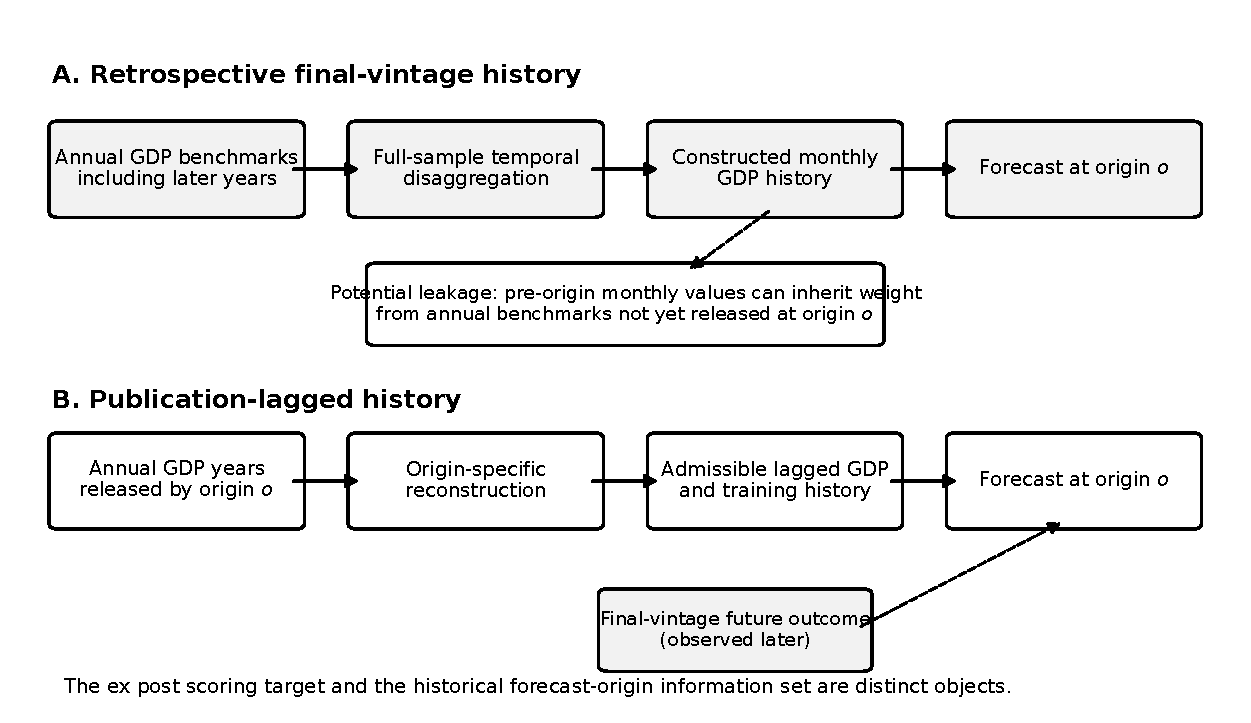
\includegraphics[width=0.96\textwidth]{Figure_Target_Information_Leakage.pdf}
\caption{Target-information leakage in retrospective versus publication-lagged forecast construction.}
\label{fig:leakage}
\begin{singlespace}\footnotesize\textit{Notes:} The retrospective path may allow unreleased annual benchmarks to influence pre-origin monthly values through temporal disaggregation. The publication-lagged path reconstructs lagged GDP and training information using only annual years permitted at the forecast origin. A final-vintage future outcome can still be used later for scoring without being treated as information available at the origin.
\end{singlespace}
\end{figure}

\subsection{Information-set admissibility and the Denton case}

The annual panel covers all 54 African economies from 2015 to 2025. The source workbook labels the annual series ``GDP (PPP)-WEO.'' Because the workbook does not identify an IMF WEO release or historical vintage, we treat the observations as final-vintage WEO-labeled benchmarks and do not infer a release vintage.

Comparable official monthly GDP releases do not exist for the full panel. For country $c$, let $Y_{cy}$ denote annual GDP-PPP and let $G^F_{ct}$ denote the final-vintage monthly path produced by additive first-difference Denton:
\begin{equation}
\min_{\{G^F_{ct}\}} \sum_{t=2}^{T} \bigl(G^F_{ct} - G^F_{c,t-1}\bigr)^2
\quad \text{subject to} \quad
\sum_{m=1}^{12} G^F_{c,y,m} = Y_{cy} \;\; \forall y.
\label{eq:denton}
\end{equation}
The evaluation target is twelve-month growth,
\begin{equation}
y^F_{ct} = 100\bigl[\log G^F_{ct} - \log G^F_{c,t-12}\bigr].
\label{eq:gdp12}
\end{equation}
The superscript $F$ marks the final-vintage path used for ex post evaluation.

For a fixed sample, Denton is a linear map from annual benchmarks to monthly values. Write
\begin{equation}
G^F = H Y^F,
\label{eq:linear_operator}
\end{equation}
where $H$ is the matrix implied by the quadratic minimization and annual aggregation constraints. At origin $t$, split the annual vector into benchmarks that are available and unavailable under the historical timing rule, $Y^F=(Y_t^A,Y_t^U)$, and partition the columns of $H$ in the same way.

A constructed path is admissible as historical information at origin $t$ only when the rows used by the forecasting model satisfy $H_{\leq t,U}=0$, or when those rows are rebuilt from $Y_t^A$ alone. If $H_{\leq t,U}\neq0$, some historical monthly values depend on annual information that had not yet been released. A forecast that uses those values as lags, or uses constructed targets in training before the benchmarks needed to form them were available, is retrospective rather than pseudo-out-of-sample.

\paragraph{Proposition 1 (interior geometric decay of Denton benchmark weights)}
Consider the additive first-difference Denton problem in equation~\eqref{eq:denton} with 12 months per annual block. Let $t=(y_0,r)$ denote month $r\in\{1,\ldots,12\}$ of year $y_0$, away from sample endpoints, and let $H_{t,y}$ be the weight of annual benchmark $Y_y$ in $G^F_t$. There are month-specific constants $C_r^+$ and $C_r^-$ such that, for every $k\geq1$,
\begin{equation}
H_{t,y_0+k}=C_r^+\mu^{k-1},\qquad
H_{t,y_0-k}=C_r^-\mu^{k-1},
\label{eq:denton_tail}
\end{equation}
with
\begin{equation}
\mu=\frac{12\sqrt{438}-289}{143}\approx-0.264745.
\label{eq:denton_mu}
\end{equation}
Thus successive off-diagonal annual weights shrink by about 73.5 percent in absolute value and reverse sign. The first unavailable-year coefficient depends on the month within the year; $0.2647$ is the ratio governing the subsequent tail, not a fixed fraction of the own-year coefficient.

The derivation reduces the Denton problem to a second-order recurrence in year-end monthly levels. The full algebra, the month-specific weight profile, and a finite-sample check for the 2015--2025 panel are reported in the online supplement. In practice, leakage is concentrated in nearby annual blocks, but its sign changes across the tail. It can strengthen or weaken a benchmark depending on the forecast origin and the data-generating process.

\subsection{Origin-specific reconstruction}

We reconstruct the GDP history separately at every forecast origin $s$. Under the baseline rule, the latest annual benchmark year allowed at the origin is
\begin{equation}
a(s)=\begin{cases}
\operatorname{year}(s)-1, & \operatorname{month}(s)\geq5,\\
\operatorname{year}(s)-2, & \operatorname{month}(s)<5.
\end{cases}
\label{eq:availyear}
\end{equation}
Only annual benchmarks through $a(s)$ enter the Denton calculation. Months after December of $a(s)$ and through the forecast origin are extrapolated using the log-monthly rate implied by the two most recent permitted annual totals,
\begin{equation}
r_{c,s}=\frac{1}{12}\bigl[\log Y_{c,a(s)}-\log Y_{c,a(s)-1}\bigr].
\label{eq:extraprate}
\end{equation}
The same release rule controls recursive training: an outcome dated in year $y$ cannot enter the estimation sample before May of $y+1$. July and November rules provide more conservative timing checks.

This is not a full historical-vintage reconstruction. Annual observations treated as already released still come from the final-vintage file. The design removes the mechanical use of future annual years; it cannot remove revisions to annual values that had already been released. We call it a publication-lagged final-vintage design rather than a real-time design.

\section{Forecasting Models and Recursive Evaluation}\label{sec:forecastdesign}

\subsection{Benchmark and GRE-augmented models}

The forecast comparison uses the same country panel, target dates, horizons, seasonal controls, and estimation scheme under both information treatments. The benchmark contains only GDP history and fixed effects. For horizon $h$,
\begin{equation}
M_0:\qquad
y^F_{c,t+h}=\alpha_c+\sum_{j=0}^{2}\phi_{j,h}y^{I(t)}_{c,t-j}
+\sum_{m=2}^{12}\delta_{m,h}\mathbf{1}\{M_{t+h}=m\}+u_{c,t+h},
\label{eq:benchmark}
\end{equation}
where $y^{I(t)}_{c,t-j}$ is twelve-month GDP growth reconstructed from the information allowed at forecast origin $t$, $\alpha_c$ is a country fixed effect, and the target-month indicators allow for seasonal differences in forecast outcomes.

The augmented model adds one variable, standardized GRE measured at the forecast origin:
\begin{equation}
M_1:\qquad
y^F_{c,t+h}=\alpha_c+\sum_{j=0}^{2}\phi_{j,h}y^{I(t)}_{c,t-j}
+\beta_h GRE_{c,t}
+\sum_{m=2}^{12}\delta_{m,h}\mathbf{1}\{M_{t+h}=m\}+v_{c,t+h}.
\label{eq:augmented}
\end{equation}
Separate coefficients are estimated for each forecast horizon. The comparison is simple: $M_0$ uses the available GDP history, while $M_1$ uses the same history plus GRE. The news variable, country set, and model form do not change between the retrospective and publication-lagged exercises.

\subsection{Recursive forecasting procedure}

Forecasts are generated one origin at a time. At each origin $t$ we first determine the annual GDP years allowed by the release rule. Those annual observations are used to rebuild the monthly GDP history through the last permitted benchmark and to extrapolate the remaining months up to $t$. We then determine which past target observations are old enough to enter the estimation sample under the same release rule. Both models are estimated on that expanding sample, forecasts are produced for $t+h$, and the origin moves forward by one month. After the target date has passed, both forecasts are scored against the same final-vintage monthly GDP outcome.

At each forecast origin we:
\begin{enumerate}
\item identify the annual GDP benchmarks available at origin $t$;
\item reconstruct the monthly GDP history that could be formed from those benchmarks;
\item admit only training outcomes permitted by the target-release rule;
\item estimate $M_0$ and $M_1$ on the same expanding sample;
\item produce the $h$-month-ahead forecasts; and
\item score both forecasts against the common final-vintage outcome after it is observed.
\end{enumerate}
The procedure is repeated for every target month from January 2020 through December 2025 and for horizons $h=1,3,6,12$.

\subsection{What changes between the two information designs}

The retrospective and publication-lagged designs are not two different forecasting models. They use the same models and the same realized target. They differ in what is treated as historically available. Table~\ref{tab:designcontrast} records that distinction.

\begin{table}[htbp]
\centering\small\singlespacing
\caption{Retrospective and publication-lagged forecast designs}
\label{tab:designcontrast}
\renewcommand{\arraystretch}{1.03}
\begin{tabularx}{\textwidth}{p{0.25\textwidth}XX}
\toprule
Element & Retrospective final-vintage design & Publication-lagged final-vintage design \\\\
\midrule
Final scoring target & Final-vintage monthly GDP path & Same final-vintage monthly GDP path \\\\
Forecast models & $M_0$ and $M_1$ & Same $M_0$ and $M_1$ \\\\
GRE predictor and scaling & Fixed GRE; 2015--2018 scaling & Same GRE and scaling \\\\
Countries and horizons & 54 countries; 1, 3, 6, 12 months & Same countries and horizons \\\\
GDP lags at forecast origin & Taken from the full final-vintage Denton history & Rebuilt from annual benchmarks permitted at the origin \\\\
Training-target entry & Realized targets treated as immediately usable & Targets enter only after the assumed annual-data release date \\\\
Estimation & Recursive expanding window & Same recursive expanding window \\\\
\bottomrule
\end{tabularx}
\end{table}

Because the models and scoring target are fixed, the 12-month change from 0.9961 to 1.0048 comes from the treatment of historical GDP information, not from changing the news measure, selecting a different set of countries, or evaluating a different outcome.

\subsection{Forecast loss and inference}

For model $j$ and horizon $h$, let $e_{j,c,t+h}$ be the forecast error. We report root mean squared forecast error,
\begin{equation}
RMSFE_j(h)=\left[\frac{1}{N_h}\sum_{c,t} e_{j,c,t+h}^2\right]^{1/2},
\end{equation}
and mean absolute error. The main comparison is the relative RMSFE,
\begin{equation}
\rho_h=\frac{RMSFE_{M_1}(h)}{RMSFE_{M_0}(h)}.
\label{eq:relative_rmsfe}
\end{equation}
Values below one favor the GRE-augmented model; values above one favor the benchmark.

Because $M_0$ is nested in $M_1$, equal-predictive-accuracy tests use the Clark--West adjusted loss differential \citep{clarkwest2007}. Forecast errors are correlated across countries and across overlapping target months. The main test averages the adjusted differential across countries within each target month and applies Newey--West HAC inference. We also report two-way covariance clustered by country and target month \citep{qu2024,akgun2024,coroneo2025}, Holm adjustment across the four horizons, and a moving-block bootstrap that resamples target months while preserving the full contemporaneous country cross-section. The one-month balanced diagnostic panel has a mean pairwise forecast-error correlation of about 0.442 and a Pesaran CD statistic of about 139.2, so independent-country inference would be inappropriate.
\section{Monte Carlo Evidence}

The simulation keeps the target-construction problem separate from the details of the African application. Each replication contains 54 economies observed monthly from 2015 through 2025. Annual GDP follows a panel process with country-specific average growth, a common annual component, and idiosyncratic shocks. The same first-difference Denton operator converts annual GDP to monthly frequency. Forecasts use three lags of twelve-month growth and country fixed effects.

We use two signal designs and one placebo. In the current-state design, the alternative variable measures the contemporaneous annual activity innovation with noise and contains no next-year innovation. The persistent-state stress design raises annual persistence and the signal-to-noise ratio so that the retrospective 12-month comparison can reverse in the same direction as the empirical application. Its parameters are not estimated from the African panel. The placebo replaces the signal with independent noise. Each design is run under the full final-vintage Denton history and under the publication-lagged rule.

\begin{table}[htbp]
\centering
\small
\caption{Monte Carlo: target-information treatment and the horizon profile of text value}
\label{tab:simulation}
\resizebox{\textwidth}{!}{%
\begin{tabular}{@{}llrrr@{}}
\toprule
DGP & Design & $h$ & Mean relative RMSFE & Share with RMSFE gain \\
\midrule
Current-state signal & Retrospective final-vintage & 1 & 1.0002 & 39.0\% \\
Current-state signal & Publication-lagged & 1 & 0.9969 & 97.7\% \\
Current-state signal & Retrospective final-vintage & 3 & 1.0002 & 36.6\% \\
Current-state signal & Publication-lagged & 3 & 0.9973 & 96.5\% \\
Current-state signal & Retrospective final-vintage & 6 & 1.0002 & 39.2\% \\
Current-state signal & Publication-lagged & 6 & 0.9987 & 84.6\% \\
Current-state signal & Retrospective final-vintage & 12 & 1.0001 & 47.5\% \\
Current-state signal & Publication-lagged & 12 & 1.0025 & 47.6\% \\
\midrule
Persistent-state stress & Retrospective final-vintage & 12 & 0.9962 & 90.2\% \\
Persistent-state stress & Publication-lagged & 12 & 1.0122 & 35.1\% \\
\bottomrule
\end{tabular}}
\begin{singlespace}\footnotesize\textit{Notes:} 1,000 replications per DGP with 54 economies and a 2015--2025 monthly calendar. The current-state signal is calibrated to a modest feasible short-horizon effect and contains no next-year innovation. The persistent-state stress DGP deliberately increases persistence and signal-to-noise to test whether retrospective final-vintage information can reproduce the direction of the empirical 12-month reversal; it is an existence calibration, not an empirical mechanism estimate. A separate pure-noise placebo remains approximately neutral under both information treatments. Full horizon results for all three DGPs appear in the online supplement.\end{singlespace}
\end{table}


\begin{figure}[htbp]
\centering
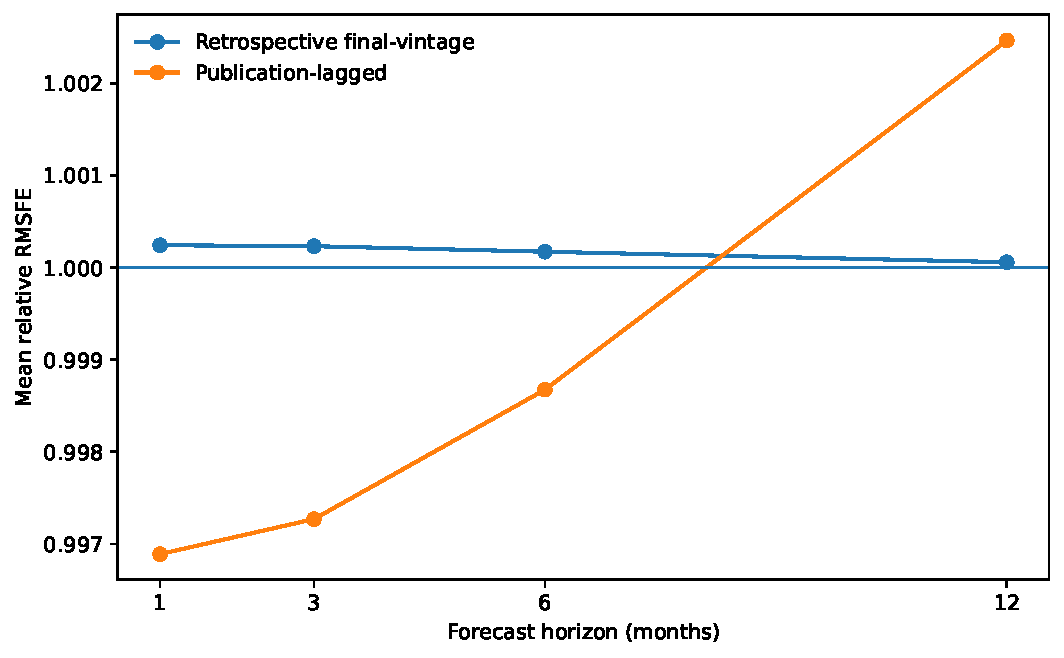
\includegraphics[width=0.76\textwidth]{Figure_Simulation_Horizon_Distortion.pdf}
\caption{Monte Carlo horizon profile under retrospective and publication-lagged target information.}
\label{fig:simulation}
\begin{singlespace}\footnotesize\textit{Notes:} Lines report mean relative RMSFE across 1,000 replications for the current-state-signal design. Values below one favor the augmented model. Full results for all three data-generating processes are reported in the online supplement.\end{singlespace}
\end{figure}

The two signal designs give different answers. In the current-state design, the one-month relative RMSFE is 1.0002 with retrospective information and 0.9969 with publication-lagged information. At twelve months both ratios are close to one. In the persistent-state stress design, the 12-month ratio is 0.9962 under the retrospective history and 1.0122 under publication timing. The placebo stays near one. The information error can hide a short-horizon gain or create a long-horizon gain. Its sign is not fixed by the Denton operator.

\section{African GDP Application and Results}

\subsection{The 12-month ranking reversal}

The earlier design used the final-vintage Denton series twice: as the realized outcome and as lagged GDP information. Under that treatment, the 12-month relative RMSFE is 0.9961. Rebuilding lagged GDP histories at each forecast origin and delaying training outcomes until the assumed release date raises the ratio to 1.0048. The model ranking changes sign.

\begin{table}[htbp]
\centering\small\singlespacing
\caption{Target-information audit: final-vintage lags versus publication-lagged lags}
\label{tab:target_audit}
\begin{tabularx}{\textwidth}{p{0.35\textwidth}rrX}
\toprule
Design & Horizon & Relative RMSFE & Interpretation \\
\midrule
Final-vintage monthly GDP treated as available at origin & 12 & 0.9961 & Retrospective diagnostic only; nominal CW $p=0.033$. \\
Publication-lagged GDP information set & 12 & 1.0048 & No long-horizon GRE gain; HAC CW $p=0.905$. \\
Publication-lagged GDP information set & 1 & 0.9964 & Modest short-horizon predictive content; HAC CW $p=0.0006$. \\
\bottomrule
\end{tabularx}
\vspace{0.35em}
\begin{minipage}{0.97\textwidth}\footnotesize\textit{Notes:} The first row reproduces the earlier working specification in which the final-vintage temporally disaggregated GDP proxy was also used as forecast-origin lag information. Because that monthly path incorporates annual benchmarks not available at historical origins, it is not used as pseudo-out-of-sample evidence in the revised paper. The corrected design uses the final-vintage series only as the realized outcome and reconstructs forecast-origin GDP information under explicit release lags.\end{minipage}
\end{table}


The correction affects both forecast-origin GDP lags and the date at which realized targets enter recursive estimation. We separate those channels with four designs. $R$ is the original retrospective design, $L$ corrects only lagged GDP, $T$ corrects only training-outcome timing, and $P$ applies both. If $\rho_d$ is GRE RMSFE divided by benchmark RMSFE under design $d$, the total change is
\[
\Delta_{P-R}=\rho_P-\rho_R.
\]
We allocate it with a two-factor Shapley calculation,
\[
\phi_{\mathrm{lag}}=\tfrac12[(\rho_L-\rho_R)+(\rho_P-\rho_T)],\qquad
\phi_{\mathrm{train}}=\tfrac12[(\rho_T-\rho_R)+(\rho_P-\rho_L)].
\]
A 5,000-draw circular moving-block bootstrap resamples 12 consecutive target months and keeps all countries together within each selected month.

\begin{table}[htbp]
\centering\small
\caption{Formal decomposition of the 12-month target-information correction}
\label{tab:channel_decomposition}
\begin{tabularx}{\textwidth}{@{}>{\raggedright\arraybackslash}Xcc@{}}
\toprule
\multicolumn{3}{l}{\textit{Panel A. Nested information-set designs}} \\
Design & Relative RMSFE & Relative MAE \\
\midrule
Retrospective: final-vintage lags + immediate training & 0.9961 & 0.9930 \\
GDP-lag corrected only & 1.0017 & 1.0070 \\
Training-timing corrected only & 0.9966 & 0.9967 \\
Fully publication-lagged & 1.0048 & 1.0122 \\
\midrule
\multicolumn{3}{l}{\textit{Panel B. Paired 12-month block-bootstrap decomposition of relative RMSFE}} \\
Contrast & Change in relative RMSFE & 95\% bootstrap interval \\
\midrule
Total correction, $P-R$ & +0.0088 & [+0.0048, +0.0171] \\
GDP-lag channel, Shapley contribution & +0.0069 & [+0.0042, +0.0145] \\
Training-timing channel, Shapley contribution & +0.0018 & [-0.0018, +0.0075] \\
\bottomrule
\end{tabularx}
\begin{minipage}{0.97\textwidth}\footnotesize\textit{Notes:} $R$ uses final-vintage GDP lags and immediate inclusion of realized training outcomes; $L$ corrects only the forecast-origin GDP lags; $T$ corrects only training-outcome availability; and $P$ applies both corrections. Panel B reports the nonlinear difference in relative RMSFE and a two-channel Shapley decomposition, so the two channel contributions sum exactly to the total $P-R$ change. The 5,000-draw circular moving-block bootstrap resamples 12-month target-date blocks and preserves the full contemporaneous cross-section. The total and GDP-lag intervals exclude zero; the training-timing interval includes zero. Complementary direct tests on country-month loss-gain differences are reported in the text and replication files.\end{minipage}
\end{table}


At twelve months, correcting only the lagged GDP history moves the ratio from 0.9961 to 1.0017. Correcting only training timing gives 0.9966. Applying both corrections gives 1.0048. The total change is $+0.0088$, with a paired block-bootstrap 95 percent interval of $[0.0048,0.0171]$. The lag-history contribution is $+0.0069$ with interval $[0.0042,0.0145]$, about 79 percent of the total. The training contribution is $+0.0018$ and its interval includes zero. Most of the reversal comes from replacing the retrospective lagged GDP history.

Figure~\ref{fig:empirical_reversal} shows the result across horizons.

\begin{figure}[htbp]
\centering
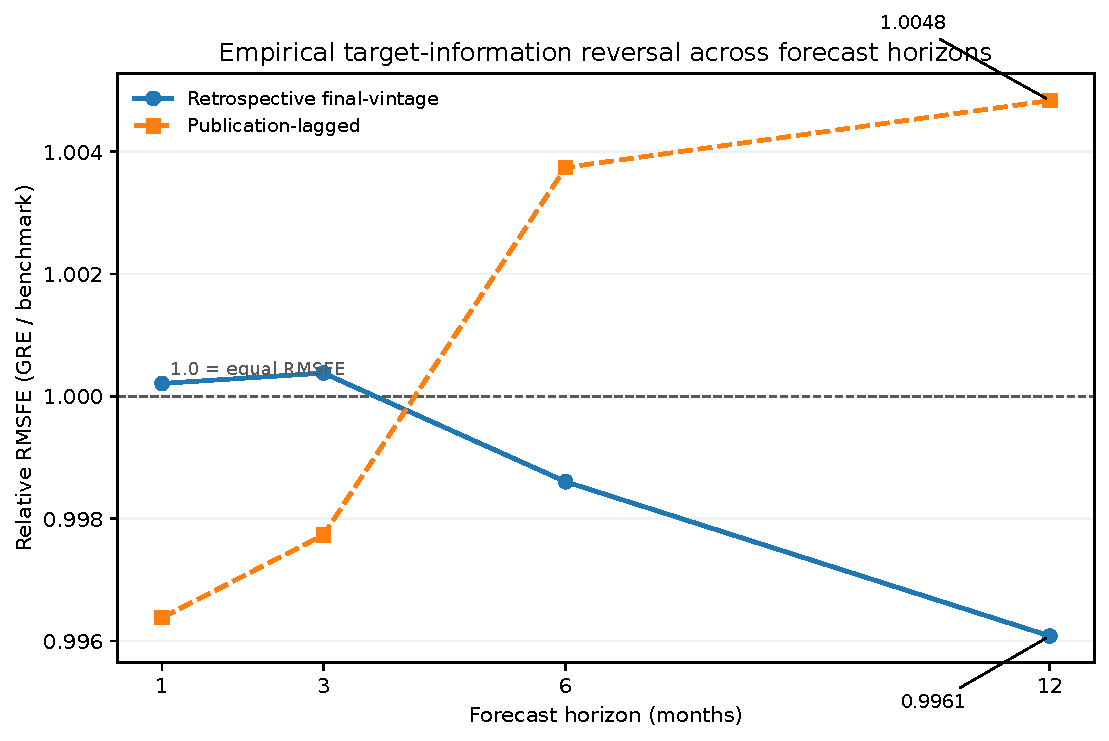
\includegraphics[width=0.82\textwidth]{Figure_Empirical_Horizon_Reversal.pdf}
\caption{Empirical horizon profile under retrospective final-vintage and publication-lagged information.}
\label{fig:empirical_reversal}
\begin{singlespace}\footnotesize\textit{Notes:} Relative RMSFE below one favors GRE. The retrospective specification uses the full final-vintage Denton history as lagged GDP information. The publication-lagged specification reconstructs forecast-origin GDP histories using only annual benchmark years permitted by the release rule.\end{singlespace}
\end{figure}

\subsection{The reversal is not a pandemic result}

The same comparison is repeated after removing all 2020--2021 forecast targets. The retrospective 12-month ratio remains below one at 0.9976, while the publication-lagged ratio rises to 1.0133. Removing the pandemic period does not explain the reversal; it makes the difference larger.

\begin{table}[htbp]
\centering
\caption{Forecast robustness excluding the 2020--2021 pandemic period}
\label{tab:excovid}
\begin{tabular}{llcccc}
\toprule
Sample & Information design & $h=1$ & $h=3$ & $h=6$ & $h=12$ \\
\midrule
2020--2025 & Retrospective & 1.0002 & 1.0004 & 0.9986 & 0.9961 \\
2020--2025 & Publication-lagged & 0.9964 & 0.9977 & 1.0037 & 1.0048 \\
2022--2025 & Retrospective & 1.0001 & 1.0002 & 0.9995 & 0.9976 \\
2022--2025 & Publication-lagged & 0.9926 & 0.9929 & 0.9988 & 1.0133 \\
\midrule
\multicolumn{6}{l}{\textit{Publication-lagged 2022--2025 inference}} \\
Horizon & Relative MAE & \multicolumn{2}{c}{CW HAC $p$} & \multicolumn{2}{c}{CW two-way $p$} \\
\midrule
1 month & 0.9863 & \multicolumn{2}{c}{$<0.001$} & \multicolumn{2}{c}{0.0271} \\
3 months & 0.9887 & \multicolumn{2}{c}{0.0014} & \multicolumn{2}{c}{0.0289} \\
6 months & 0.9978 & \multicolumn{2}{c}{0.0811} & \multicolumn{2}{c}{0.1583} \\
12 months & 1.0229 & \multicolumn{2}{c}{0.9697} & \multicolumn{2}{c}{0.7706} \\
\bottomrule
\end{tabular}
\begin{minipage}{0.97\textwidth}\footnotesize\textit{Notes:} Entries in the first panel are GRE RMSFE divided by the corresponding benchmark RMSFE. The restricted evaluation sample begins in January 2022 and ends in December 2025, removing all 2020--2021 forecast targets while retaining the same recursive estimation history and information-set rules. The publication-lagged 12-month ratio remains above one after the exclusion, whereas the retrospective ratio remains below one. The one- and three-month publication-lagged comparisons strengthen in the restricted sample. Clark--West values are one-sided tests of incremental predictive content, with target-month HAC and complementary country$\times$target-month two-way covariance.\end{minipage}
\end{table}


The release month is also uncertain across 54 economies. Repeating the reconstruction with July and November availability leaves the one-month point estimates close to the May result. At one month, relative RMSFE is 0.9964 under May, 0.9969 under July, and 0.9973 under November. The 12-month conclusion remains unfavorable under the corrected design. The release-calendar exercise is a timing sensitivity check, not a claim that every country publishes annual GDP on the same date.

\begin{table}[htbp]
\centering\small
\caption{Sensitivity of the one-month GRE result to annual-data release timing}
\label{tab:release_timing}
\resizebox{\textwidth}{!}{%
\begin{tabular}{lrrrrrr}
\toprule
Annual year $y$ usable from & Rel. RMSFE & Rel. MAE & HAC CW $p$ & Two-way $p$ & Bootstrap CW $p$ & Countries $<1$ \\
\midrule
May of $y+1$ & 0.9964 & 0.9897 & 0.0006 & 0.053 & 0.037 & 33/54 \\
July of $y+1$ & 0.9969 & 0.9894 & 0.0004 & 0.039 & 0.038 & 31/54 \\
November of $y+1$ & 0.9973 & 0.9910 & 0.0001 & 0.030 & 0.019 & 32/54 \\
\bottomrule
\end{tabular}}
\vspace{0.35em}
\begin{minipage}{0.97\textwidth}\footnotesize\textit{Notes:} Each row reconstructs the GDP information set and recursive training eligibility under the stated release convention. Bootstrap results use 5,000 moving-block replications with 12-month target-date blocks and preserve the contemporaneous country cross-section.\end{minipage}
\end{table}


\subsection{What remains at short horizons}

Under the baseline publication rule, the one-month benchmark RMSFE is 8.375 and the GRE RMSFE is 8.344, giving relative RMSFE 0.9964. Relative MAE is 0.9897. At three months the RMSFE ratio is 0.9977; at six months it is 1.0037; at twelve months it is 1.0048.

\begin{table}[htbp]
\centering\scriptsize
\caption{Publication-lagged forecast performance of the GRE-augmented model}
\label{tab:main_results}
\resizebox{\textwidth}{!}{%
\begin{tabular}{rrrrrrrr}
\toprule
$h$ & Benchmark RMSFE & GRE RMSFE & Rel. RMSFE & Benchmark MAE & GRE MAE & HAC CW $p$ & Two-way $p$ \\
\midrule
1  & 8.375 & 8.344 & 0.9964 & 5.441 & 5.385 & 0.0006 & 0.053 \\
3  & 8.493 & 8.473 & 0.9977 & 5.523 & 5.483 & 0.041 & 0.084 \\
6  & 8.588 & 8.620 & 1.0037 & 5.513 & 5.529 & 0.878 & 0.869 \\
12 & 19.264 & 19.357 & 1.0048 & 7.028 & 7.114 & 0.905 & 0.872 \\
\bottomrule
\end{tabular}}
\vspace{0.35em}
\begin{minipage}{0.97\textwidth}\footnotesize\textit{Notes:} The dependent variable is final-vintage twelve-month GDP-PPP proxy growth. Forecast-origin GDP lags and the recursive training sample obey the baseline May release rule described in Table~\ref{tab:design}. Relative RMSFE below one indicates lower forecast loss. Holm adjustment across the four target-month HAC tests gives adjusted $p=0.0023$ at $h=1$ and $p=0.122$ at $h=3$. The corresponding two-way adjusted values are 0.211 and 0.253.\end{minipage}
\end{table}


The one-month Clark--West result is strong under target-month HAC inference ($p=0.0006$) and weaker under two-way clustering ($p=0.053$). A 5,000-draw moving-block bootstrap gives a one-sided Clark--West value of 0.037, but the 95 percent interval for the raw percentage RMSFE improvement is approximately $[-0.50,1.44]$. Country results are mixed: 33 of 54 economies have lower one-month RMSFE with GRE and 21 do not. After removing 2020--2021, the one-month ratio improves to 0.9926.

The online supplement reports three checks on this short-horizon result. Exact-text deduplication changes the one-month ratio only from 0.9964 to 0.9969. Splitting forecast origins by the age of the annual information set gives suggestive results under the May and July conventions but not under November, and a direct regression of loss improvement on information age is weak. GRE also does not significantly predict the revision from the publication-lagged current-growth estimate to final-vintage growth. We do not assign a causal mechanism to the one-month result.

\subsection{A richer conventional benchmark}

We next replace the parsimonious benchmark with a panel of up to 162 monthly macroeconomic series: publication-lagged GDP growth, inflation, and exchange-rate depreciation for each economy. After removing series with limited pre-evaluation coverage or negligible variance, 159 remain. Means, standard deviations, and principal-component loadings are estimated only on March 2016--December 2018 and then frozen. Six factors explain 82.1 percent of calibration-sample variance.

\begin{table}[htbp]
\centering\scriptsize
\caption{One-month GRE comparison against a wide macroeconomic factor benchmark}
\label{tab:wide_factor}
\resizebox{\textwidth}{!}{%
\begin{tabular}{lrrrrrr}
\toprule
Benchmark information & Benchmark RMSFE & +GRE RMSFE & Rel. RMSFE & Rel. MAE & HAC CW $p$ & Two-way $p$ \\
\midrule
Pooled AR, publication-lagged GDP lags & 8.375 & 8.344 & 0.9964 & 0.9897 & 0.0006 & 0.053 \\
Wide factors, macro variables lagged 1 month & 9.325 & 9.313 & 0.9987 & 0.9946 & 0.112 & 0.148 \\
Wide factors, macro variables lagged 2 months & 9.875 & 9.881 & 1.0006 & 0.9972 & 0.451 & 0.457 \\
\bottomrule
\end{tabular}}
\vspace{0.35em}
\begin{minipage}{0.97\textwidth}\footnotesize\textit{Notes:} The wide information set contains 162 candidate monthly series: publication-lagged GDP growth, inflation, and exchange-rate depreciation for 54 economies. Series with fewer than 24 observations in the 2016:03--2018:12 calibration window or negligible variance are removed, leaving 159. Means, standard deviations, and PCA loadings are frozen before evaluation. Six components are retained because they are the minimum needed to exceed 80 percent of pre-evaluation variance (82.1 percent). The wide factor benchmark is data-rich but has higher absolute RMSFE than the parsimonious AR benchmark. The inflation and exchange-rate series are supplied final-vintage macro data without archived release vintages, so one- and two-month lags are used as timing safeguards rather than claimed real-time vintages. GRE's small incremental improvement is not statistically significant against this benchmark.\end{minipage}
\end{table}


With a one-month macro lag, adding GRE to the factor benchmark gives relative RMSFE 0.9987 and relative MAE 0.9946. The target-month HAC and two-way Clark--West values are 0.112 and 0.148. With a two-month macro lag, relative RMSFE is about one. The small one-month GRE result is sensitive to how much conventional information is placed in the benchmark. The 12-month information-set reversal is not.

\begin{figure}[htbp]
\centering
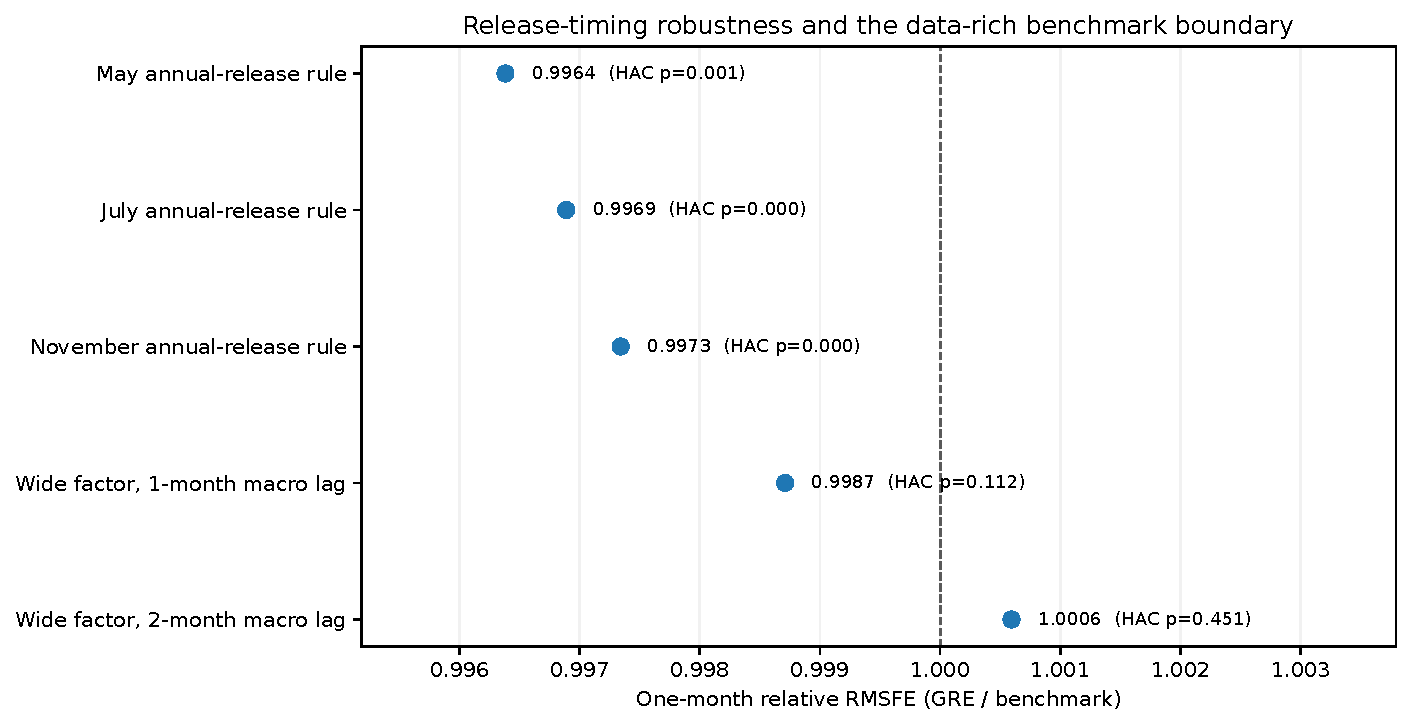
\includegraphics[width=0.90\textwidth]{Figure_Release_Benchmark_Boundary.pdf}
\caption{Release-timing robustness and the data-rich benchmark boundary at the one-month horizon.}
\label{fig:release_benchmark}
\begin{singlespace}\footnotesize\textit{Notes:} Points report relative RMSFE for GRE versus the corresponding benchmark. The first three rows vary the assumed annual GDP release month under the parsimonious publication-lagged benchmark. The final two rows augment the conventional information set with six principal components extracted from 159 retained macroeconomic series. Parenthetical values are target-month HAC Clark--West $p$-values.\end{singlespace}
\end{figure}

\FloatBarrier
\section{Conclusion}

A constructed high-frequency target can be perfectly suitable for ex post scoring and still be unsuitable as historical information. The difference is timing. If an annual benchmark was not available at a forecast origin, monthly values that depend on that benchmark should not enter lagged regressors or recursive training at that origin.

For additive first-difference Denton, the dependence on neighboring annual benchmarks can be described analytically. Once the off-diagonal tail begins, successive annual weights decay by about 0.2647 in absolute value and alternate in sign. The effect on relative forecast loss has no fixed direction, which is also what the simulations show.

In the African GDP application, correcting the historical information set changes the model ranking. The 12-month relative RMSFE is 0.9961 when the final-vintage Denton history is treated as if it had been available at every forecast origin. It is 1.0048 when GDP lags and recursive training obey the publication-timing rule. Removing 2020--2021 changes the comparison from 0.9976 to 1.0133. The paired decomposition assigns most of the difference to the lagged GDP history rather than to delayed entry of training outcomes.

The application is not a full real-time exercise. The annual GDP file is final-vintage, and the May, July, and November rules cannot remove later revisions to annual observations that are treated as already released. Country-specific historical release calendars are also unavailable. A stronger real-time replication would require archived annual vintages and actual release dates for each country.

The small one-month GRE gain should also be read narrowly. It is mixed across countries and weakens against the data-rich factor benchmark. That does not affect the target-information result. For forecast evaluation, the practical point is this: when the target has been reconstructed from lower-frequency data, the historical path used by the forecasting model needs its own information-set audit.
\section*{Acknowledgments}
None.

\paragraph{Funding} This research did not receive any specific grant from funding agencies in the public, commercial, or not-for-profit sectors.

\section*{Conflict of Interest}
The authors declare that they have no known competing financial interests or personal relationships that could have appeared to influence the work reported in this paper.

\section*{Data Availability Statement}
The data and replication materials that support the findings of this study are available from the corresponding author upon reasonable request. The full underlying news-article archive cannot be redistributed because it contains third-party copyrighted material. The source registry, derived country-month indicators, scoring documentation, code, constructed GDP series, and forecast-evaluation outputs can be provided on request.

\begingroup
\small
\setlength{\bibsep}{0pt plus 0.2ex}
\begin{thebibliography}{99}

\bibitem[Abeyie(2026)]{abeyie2026}
Abeyie, G. A. (2026). Beyond news headlines and TF-IDF: Enhancing text-based
forecasting models with validated collocations and improved attention.
\emph{International Journal of Forecasting, 42}, 752--773.
\url{https://doi.org/10.1016/j.ijforecast.2025.09.002}

\bibitem[Ad{\"a}mmer et al.(2025)]{adaemmer2025}
Ad{\"a}mmer, P., Pr{\"u}ser, J., \& Sch{\"u}ssler, R. A. (2025). Forecasting
macroeconomic tail risk in real time: Do textual data add value?
\emph{International Journal of Forecasting, 41}, 307--320.
\url{https://doi.org/10.1016/j.ijforecast.2024.05.007}

\bibitem[Ahir et al.(2022)]{ahir2022}
Ahir, H., Bloom, N., \& Furceri, D. (2022). The World Uncertainty Index.
NBER Working Paper 29763. \url{https://doi.org/10.3386/w29763}

\bibitem[Akgun et al.(2024)]{akgun2024}
Akgun, O., Pirotte, A., Urga, G., \& Yang, Z. (2024). Equal predictive ability
tests based on panel data with applications to OECD and IMF forecasts.
\emph{International Journal of Forecasting, 40}, 202--228.
\url{https://doi.org/10.1016/j.ijforecast.2023.02.001}

\bibitem[Ardia and Bluteau(2026)]{ardia2026}
Ardia, D., \& Bluteau, K. (2026). Optimal text-based time-series indices.
\emph{International Journal of Forecasting, 42}, 44--60.
\url{https://doi.org/10.1016/j.ijforecast.2025.07.003}

\bibitem[Bae(2024)]{bae2024}
Bae, J. (2024). Factor-augmented forecasting in big data.
\emph{International Journal of Forecasting, 40}, 1660--1688.
\url{https://doi.org/10.1016/j.ijforecast.2024.02.004}

\bibitem[Baker et al.(2016)]{baker2016}
Baker, S. R., Bloom, N., \& Davis, S. J. (2016). Measuring economic policy
uncertainty. \emph{The Quarterly Journal of Economics, 131}, 1593--1636.
\url{https://doi.org/10.1093/qje/qjw024}

\bibitem[Ba{\'n}bura et al.(2013)]{banbura2013}
Ba{\'n}bura, M., Giannone, D., Modugno, M., \& Reichlin, L. (2013).
Now-casting and the real-time data flow. In G. Elliott \& A. Timmermann
(Eds.), \emph{Handbook of Economic Forecasting} (Vol. 2A, pp. 195--237).
Elsevier. \url{https://doi.org/10.1016/B978-0-444-53683-9.00004-9}

\bibitem[Bok et al.(2018)]{bok2018}
Bok, B., Caratelli, D., Giannone, D., Sbordone, A. M., \& Tambalotti, A.
(2018). Macroeconomic nowcasting and forecasting with big data. \emph{Annual
Review of Economics, 10}, 615--643.
\url{https://doi.org/10.1146/annurev-economics-080217-053214}

\bibitem[Caldara and Iacoviello(2022)]{caldara2022}
Caldara, D., \& Iacoviello, M. (2022). Measuring geopolitical risk.
\emph{American Economic Review, 112}, 1194--1225.
\url{https://doi.org/10.1257/aer.20191823}

\bibitem[Chow and Lin(1971)]{chowlin1971}
Chow, G. C., \& Lin, A. (1971). Best linear unbiased interpolation, distribution, and extrapolation of time series by related series.
\emph{The Review of Economics and Statistics, 53}(4), 372--375.
\url{https://doi.org/10.2307/1928739}

\bibitem[Clark and West(2007)]{clarkwest2007}
Clark, T. E., \& West, K. D. (2007). Approximately normal tests for equal
predictive accuracy in nested models. \emph{Journal of Econometrics, 138},
291--311. \url{https://doi.org/10.1016/j.jeconom.2006.05.023}

\bibitem[Coroneo and Iacone(2025)]{coroneo2025}
Coroneo, L., \& Iacone, F. (2025). Testing for equal predictive accuracy with
strong dependence. \emph{International Journal of Forecasting, 41},
1073--1092. \url{https://doi.org/10.1016/j.ijforecast.2024.11.003}

\bibitem[Croushore(2006)]{croushore2006}
Croushore, D. (2006). Forecasting with real-time macroeconomic data. In
G. Elliott, C. W. J. Granger, \& A. Timmermann (Eds.), \emph{Handbook of
Economic Forecasting} (Vol. 1, pp. 961--982). Elsevier.
\url{https://doi.org/10.1016/S1574-0706(05)01017-7}

\bibitem[Croushore and Stark(2001)]{croushorestark2001}
Croushore, D., \& Stark, T. (2001). A real-time data set for macroeconomists.
\emph{Journal of Econometrics, 105}, 111--130.
\url{https://doi.org/10.1016/S0304-4076(01)00072-0}

\bibitem[Denton(1971)]{denton1971}
Denton, F. T. (1971). Adjustment of monthly or quarterly series to annual
totals: An approach based on quadratic minimization. \emph{Journal of the
American Statistical Association, 66}, 99--102.
\url{https://doi.org/10.1080/01621459.1971.10482227}

\bibitem[Eilers(2003)]{eilers2003}
Eilers, P. H. C. (2003). A perfect smoother. \emph{Analytical Chemistry, 75},
3631--3636. \url{https://doi.org/10.1021/ac034173t}

\bibitem[Feng(2009)]{feng2009}
Feng, H. (2009). Real-time or current vintage: Does the type of data matter for
forecasting and model selection? \emph{Journal of Forecasting, 28}, 183--193.
\url{https://doi.org/10.1002/for.1089}

\bibitem[Fern\'{a}ndez(1981)]{fernandez1981}
Fern\'{a}ndez, R. B. (1981). A methodological note on the estimation of time series.
\emph{The Review of Economics and Statistics, 63}(3), 471--476.
\url{https://doi.org/10.2307/1924371}

\bibitem[Gentzkow et al.(2019)]{gentzkow2019}
Gentzkow, M., Kelly, B., \& Taddy, M. (2019). Text as data. \emph{Journal of
Economic Literature, 57}, 535--574.
\url{https://doi.org/10.1257/jel.20181020}

\bibitem[Giannone et al.(2008)]{giannone2008}
Giannone, D., Reichlin, L., \& Small, D. (2008). Nowcasting: The real-time
informational content of macroeconomic data. \emph{Journal of Monetary
Economics, 55}, 665--676.
\url{https://doi.org/10.1016/j.jmoneco.2008.05.010}

\bibitem[International Monetary Fund(2017)]{imfqna2017}
International Monetary Fund. (2017). \emph{Quarterly national accounts manual: 2017 edition}. International Monetary Fund.

\bibitem[Kim and Swanson(2018)]{kimswanson2018}
Kim, H. H., \& Swanson, N. R. (2018). Methods for backcasting, nowcasting and forecasting using factor-MIDAS: With an application to Korean GDP.
\emph{Journal of Forecasting, 37}(3), 281--302.
\url{https://doi.org/10.1002/for.2499}

\bibitem[Litterman(1983)]{litterman1983}
Litterman, R. B. (1983). A random walk, Markov model for the distribution of time series.
\emph{Journal of Business \& Economic Statistics, 1}(2), 169--173.
\url{https://doi.org/10.1080/07350015.1983.10509336}

\bibitem[Pfarrhofer(2024)]{pfarrhofer2024}
Pfarrhofer, M. (2024). Forecasts with Bayesian vector autoregressions under real time conditions.
\emph{Journal of Forecasting, 43}(3), 771--801.
\url{https://doi.org/10.1002/for.3055}

\bibitem[Qu et al.(2024)]{qu2024}
Qu, R., Timmermann, A., \& Zhu, Y. (2024). Comparing forecasting performance
with panel data. \emph{International Journal of Forecasting, 40}, 918--941.
\url{https://doi.org/10.1016/j.ijforecast.2023.08.001}

\bibitem[R{\"u}nstler et al.(2009)]{ruenstler2009}
R{\"u}nstler, G., Barhoumi, K., Benk, S., Cristadoro, R., Den Reijer, A.,
Jakaitiene, A., Jelonek, P., Rua, A., Ruth, K., \& Van Nieuwenhuyze, C. (2009).
Short-term forecasting of GDP using large datasets: A pseudo real-time forecast
evaluation exercise. \emph{Journal of Forecasting, 28}, 595--611.
\url{https://doi.org/10.1002/for.1105}

\bibitem[Seo(2025)]{seo2025}
Seo, B. (2025). Econometric forecasting using ubiquitous news text:
Text-enhanced factor model. \emph{International Journal of Forecasting, 41},
1055--1072. \url{https://doi.org/10.1016/j.ijforecast.2024.11.001}

\bibitem[Stock and Watson(2002)]{stockwatson2002}
Stock, J. H., \& Watson, M. W. (2002). Macroeconomic forecasting using
diffusion indexes. \emph{Journal of Business \& Economic Statistics, 20},
147--162. \url{https://doi.org/10.1198/073500102317351921}

\bibitem[Stock and Watson(2004)]{stockwatson2004}
Stock, J. H., \& Watson, M. W. (2004). Combination forecasts of output growth
in a seven-country data set. \emph{Journal of Forecasting, 23}, 405--430.
\url{https://doi.org/10.1002/for.928}

\bibitem[Timmermann(2006)]{timmermann2006}
Timmermann, A. (2006). Forecast combinations. In G. Elliott,
C. W. J. Granger, \& A. Timmermann (Eds.), \emph{Handbook of Economic
Forecasting} (Vol. 1, pp. 135--196). Elsevier.
\url{https://doi.org/10.1016/S1574-0706(05)01004-9}

\bibitem[Zheng et al.(2024)]{zheng2024}
Zheng, T., Fan, X., Jin, W., \& Fang, K. (2024). Words or numbers?
Macroeconomic nowcasting with textual and macroeconomic data.
\emph{International Journal of Forecasting, 40}, 746--761.
\url{https://doi.org/10.1016/j.ijforecast.2023.05.006}

\end{thebibliography}
\endgroup


\end{document}
